\section{绪论}
\setcounter{page}{1}
这里是一段内容,这里是一段内容,这里是一段内容,这里是一段内容,这里是一段内容,这里是一段内容,这里是一段内容,这里是一段内容,这里是一段内容,这里是一段内容,这里是一段内容,这里是一段内容,这里是一段内容。

这里也是一段内容,这里也是一段内容,这里也是一段内容,这里也是一段内容,这里也是一段内容,这里也是一段内容,这里也是一段内容,这里也是一段内容,这里也是一段内容,这里也是一段内容,这里也是一段内容,这里也是一段内容。

\subsection{引言}
这是2级章节的内容。

\subsubsection{基本术语}
这是3级章节的内容。



\subsection{假设空间}
这里是表\ref{tab.housing-price}的用法。

\begin{table}[H]
    \centering
    \caption{\label{tab.housing-price}房价预测}
    \begin{tabular}{ccc}
        \toprule
        年份&学校数量&房价\\
        \midrule 
        2020&1所&1万/$m^2$\\
        \hline
        2021&2所&4万/$m^2$\\
        \bottomrule
    \end{tabular}
\end{table}

这里是图\ref{fig.roc}的用法。\par
\begin{figure}[h]
\centering
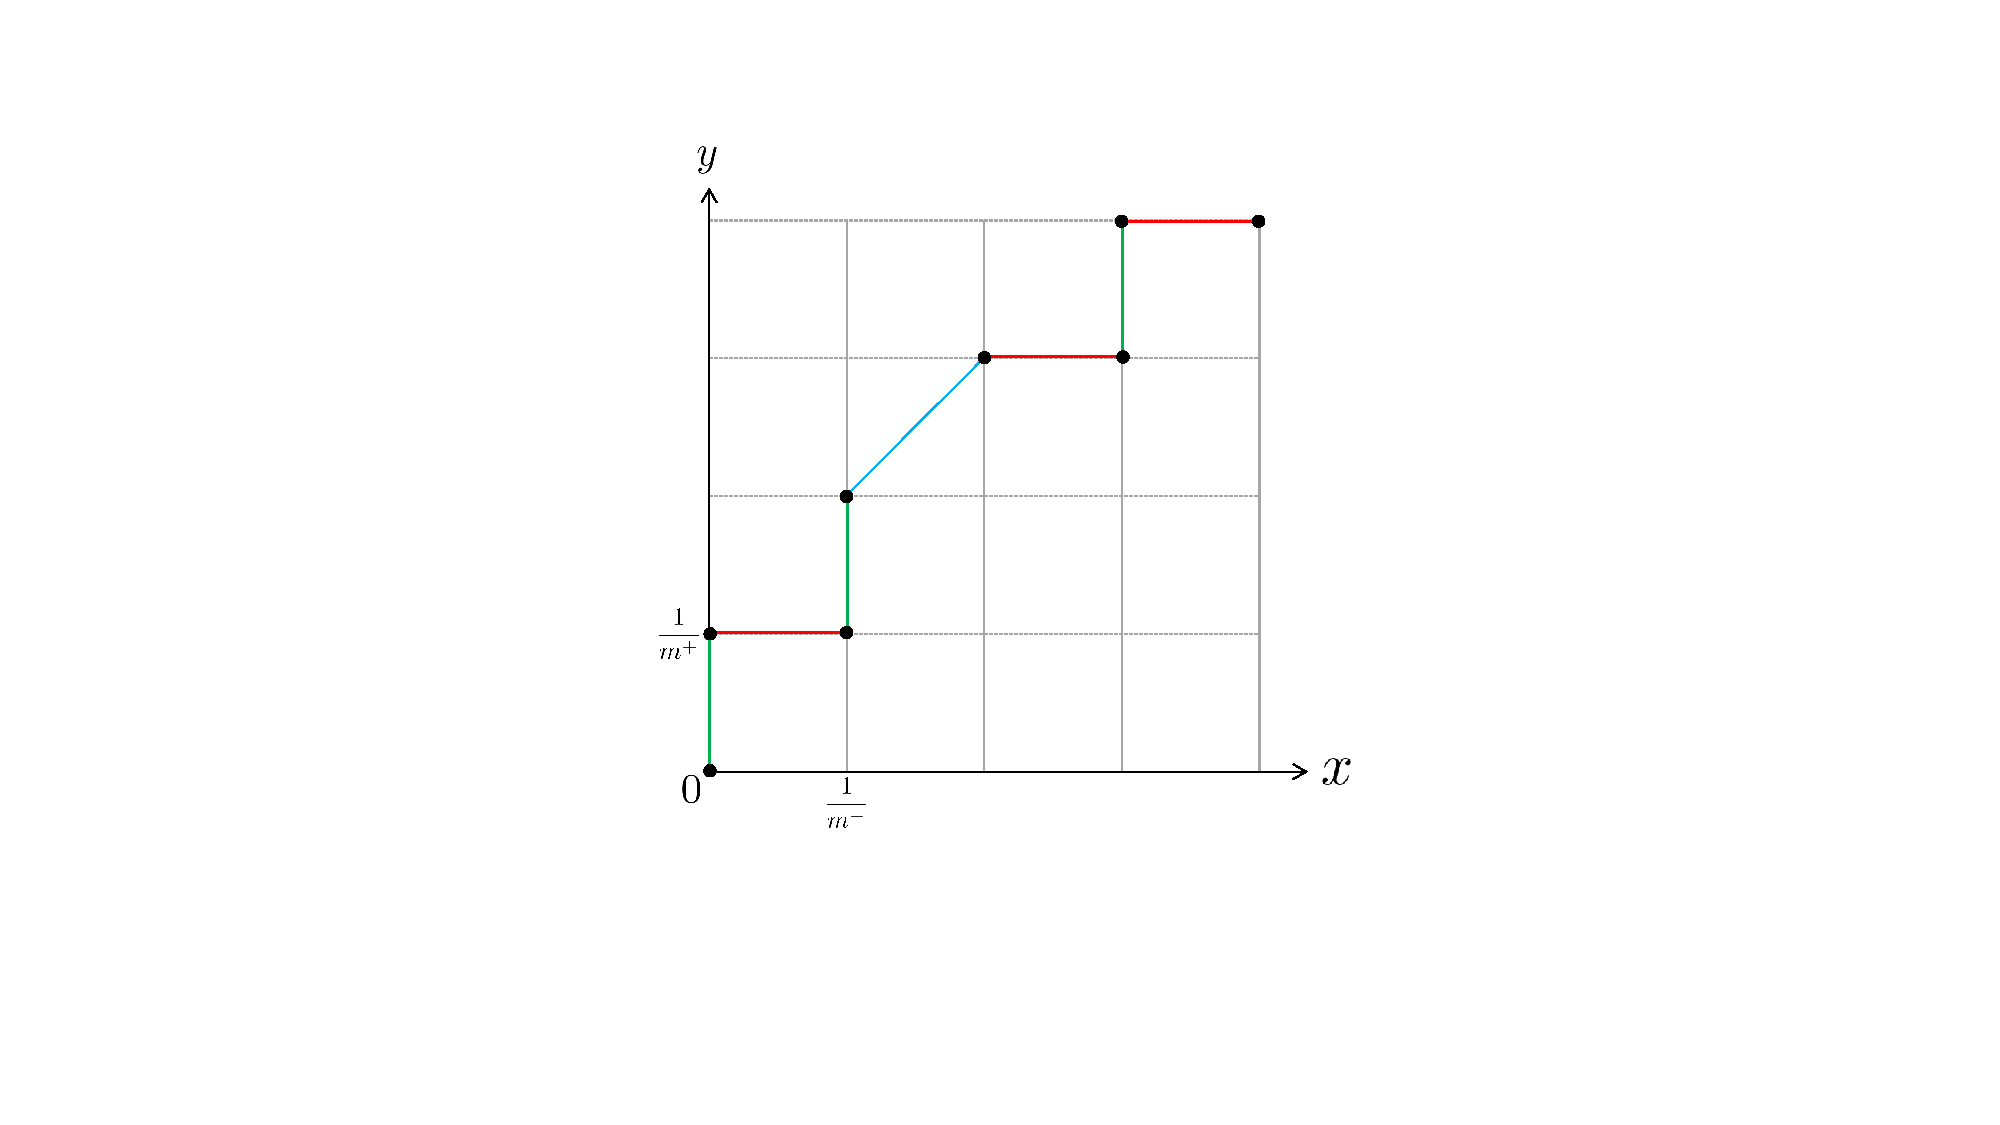
\includegraphics[trim=0 123 0 123,scale=0.5]{resources/ch1/roc.pdf}
\caption{ROC曲线示意}
\label{fig.roc}
\end{figure}

这里是正常引用参考文献\cite{chenxiru},这里是上角标引用参考文献\upcite{chenxiru}。

\bibliographystyle{unsrt}
\bibliography{ref.bib}